Wavelets evolved from atomic function theory where they were developed
as basic atoms or building blocks of all functions. This chapter
provides an overview of wavelets. This is done first by providing the
standard definitions and concepts of the wavelet basis function, the
wavelet transform and multiresolution representation. Then a numerical
example is utilized to demonstrate the concepts. The next section
details the numerical implementation of the wavelet transform. The
last section represents the 2D wavelet transform.

\section{The Wavelet Basis Function}

This section provides the basic properties of a wavelet function. It
first describes some general properties of functions. Then it presents
the translation and dilation properties which can be used to build an
entire bases. Finally, it presents the wavelet function itself.

\subsection{Function Properties}

There are a number of different properties that can be used to
classify functions. These include integrability, symmetry, compactness
and orthogonality. The properties will be introduced now and used in
the rest of the chapter.

A function, $f(\cdot)$, is {\it square integrable} if its $L_2$ norm is finite. This can be
expressed by
\[ 
f(x) \in L_2({\mathbb R}) \ \mbox{ if } \ \int\limits _{-\infty}^{\infty} \left|f(x)\right|^2 dx < \infty.
\]
A one-dimensional function is {\it symmetric} about the $y$-axis if 
\[
f(x) = f(-x)
\]
and it is {\it antisymmetric} if
\[
f(x) = -f(-x).
\]
The term symmetric is synonymous with ``even function.''  Likewise, antisymmetric is synonymous with ``odd functions.''

A set is considered {\it compact} in the $n$-dimensional real space,
${\mathbb R}^n$ if it is both closed and bounded. A function has {\it
compact support} if it is zero outside of a compact set. This implies that
there exists $n$-dimensional sphere, $S^n$, where 
\[
f(x) = 0 \qquad \forall x \not \in S^n.
\]

Orthogonality is another concept necessary for this thesis.  Two different basis functions are {\it orthogonal} if their inner product is zero.  The inner product of two functions, $f$ and $g$, can be represented by
\[
\left< f, g \right> = \int_{-\infty}^\infty f(x)g(x) \ dx.
\]
They are {\it orthonormal} if they are both orthogonal and have a norm of one.

\subsection {Translation and Dilation}

Translation shifts the basis function along the variable axis. The translation of a function, $f$, can be represented by $f_k$ where
\[
f_k(t) = f(t-k).
\]
Notice that translation does not alter the shape of the function, only the position of the function along the number space of $t$ \cite{translation}.

Dilation (also called contraction) transforms a one-dimensional function in width, and the output in height.   The dilation of a function, $f$, can be presented by $f_{j}$ where
\[
f_\alpha(t) = f(\alpha t).
\]
If $\alpha<1$ then the width of the function is increased. Otherwise it is decreased. 

Often, a scaling value is associated with the dilation operation.  An arbitrary form of this scaling is defined with $s$ as follows:
\[
f_s (t) = s f(t) 
\]
If $s>1$ then the height of the function is increased.   Likewise, when $s<1$ the height is decreased.  Often the scaling component is included in either translation, dilation or both.  In orthonormal-translation-dilation, there is a special case of notation as described next. 

These definitions can be combined into the translation-dilation representation upon dyadic intervals. A function $f$ can be expressed by a dilation of $j$ and a translation of $k$ through
\[
f_{j,k}(t) = 2^{j/2}f(2^jt-k) \qquad \forall j, k \in {\mathbb Z}.
\]
There is a special case for including the scaling factor of $2^{j/2}$.  The scaling value $2^{j/2}$ is applied to force a dyadic orthonormal condition.  
A function is said to have the orthonormal translation-dilation property when for two translation-dilations, $f_{j,k}$ and $f_{l,m}$, the result can be expressed by \cite{ChuiIntro}
\[
\left< f_{j,k} , f_{l,m} \right> = \delta_{j,l} \delta_{k,m}.
\]

\subsection {The Wavelet Basis Function}

The two mandatory properties of a wavelet basis function are:
\begin{itemize}
\item it must square integrable,   and
\item must have a zero average, i.e.:
\[
\int_{-\infty}^{+\infty}\psi(x) \ dx = 0.
\]
\end{itemize}
In addition, the class of orthogonal wavelet basis functions are restricted to satisfy
the orthonormal translation-dilation property. This restriction no longer applies to all wavelets by the lifting scheme % hasbeen removed through the lifting scheme 
\cite{fernandez96software}. An example
of a strict definition of a wavelet is given by Charles Chui \cite{ChuiIntro} (page 61):  
\begin{quote}
``A function $\psi \in L_2({\mathbb R})$ is called an orthonormal wavelet if the family $\{\psi_{j,k}\}$ defined 
\[ \psi_{j,k}(x)  = 2^{j/2} \psi (2 ^j x -k) \forall j,k \in {\mathbb Z} \]
is an orthonormal basis of $L_2({\mathbb R})$ where $\langle \psi _{j,k} , \psi_{l,m} \rangle = \delta _{j,l} \delta_{k,m}$,  $ \forall j,k,l,m\in {\mathbb Z}$ and every $ f\in L_2({\mathbb R})$ can be written as 
\[ f(x)= \sum\limits _{j,k = -\infty}^{\infty} c_{j,k} \psi _{j,k} (x)  \]
where the series convergences and is %of the series 
%\[ f(x) = \sum\limits _{j,k = -\infty}^{\infty}  c_{j,k} \psi _{j,k} (x)  \]
in $L_2({\mathbb R})$ such that 
\[ \lim\limits _{M_1, M_2, N_1 , N_2} || f - \sum\limits _{j=-M_2}^{N_2} \sum\limits _{k=-M_1}^{N_1} c_{j,k} \psi _{j,k} || = 0 \]
The simplest example of orthonormal wavelets is the Haar Transform.''
\end{quote}

There is more than one wavelet basis function. Additional classifications used include the symmetry and compactness \cite{jawerth94overview}. The Haar Wavelet Basis function actually fulfills the strictest definition of a wavelet basis function, and has additional properties.  The Haar Wavelet Basis Function has compact support.  It is also symmetric.  Furthermore, it has been stated by Walker\cite{walker}, Gregory Beylkin \cite{amsbeylkin,bvpbeylkin,fwtnal} and Chui \cite{ChuiIntro} that the Haar Wavelet Basis Function is the only wavelet basis function in $L_2({\mathbb R})$ that is orthogonal, compact, and symmetric.  The Haar wavelet basis function is defined below.
\begin{equation} \label{eqn:waveletbasis}
\psi(x) = \left\{
\begin{array}{cc}
1 & 0\le x < \frac{1}{2} \\
-1 & \frac{1}{2} \le x < 1 \\
0 & {otherwise}
\end{array}\right. 
\end{equation}


\section{The Wavelet Transform}

The wavelet transform is comprised of two parts, an average sample and
a difference sample. This is expressed by first looking at pairs of
wavelets and then looking at the actual representation.

\subsection {Wavelet Pairs: The Averaging Basis Function}

The Wavelet Basis Function section defined the Haar Wavelet Basis
Function defined the Haar Wavelet Basis function, in equation
\ref{eqn:waveletbasis}.  However, there exists a concept of a wavelet
pair.  These pairs exist as averaging and differencing basis.  The
wavelet basis function and differencing basis are synonymous.  The
averaging basis concept was derived from classic multi-resolution
which is described in section \ref{sec:multiresolution}.

This section only defines the wavelet basis pair in terms of a wavelet
averaging basis and shows an example with the Haar Averaging Basis
Function.  A wavelet pair is a set of two basis functions containing
one wavelet basis function and one averaging basis function which meet
the following criteria:
\begin{itemize}
\item both must be square integrable, 
\item both must satisfy the orthonormal dyadic translation-dilation property, and
\item the wavelet basis function must be orthogonal with the average basis function.
\end{itemize}
The simplest form of the averaging filter is the Haar Averaging
Filter, and it is a pair to the Haar Wavelet Basis Function.  Like the
Haar Wavelet Basis Function, the Haar Averaging Filter also satisfies
the dyadic-orthogonal translation property and is in $L_2({\mathbb R})$ The
mother \cite{walker,victor,ChuiIntro,tabor,graps} function for the Haar Averaging Filter is defined by
\[
\phi(x) =
\left\{\begin{array}{cc}1 & 0\le x < 1 \\0 &
{otherwise.}\end{array}\right.
\]

\subsection{Transform Representation}

This derivation uses the wavelet pair to define the wavelet transform.
Any wavelet transform uses a satisfactory wavelet pair to transform an
array into two halves which constitute the average filter sub-array
and the difference filtered sub-array.  This definition commonly
refers to the average filtered sub-array as the average terms and
difference terms, respectively.  The concatenated array of average and
difference terms constitutes a similar array to the original array,
and the same properties as similar vectors.  Also, for every wavelet
transform there is a straightforward method to restore the original
array from the wavelet transformed array called the inverse wavelet
transform.

One form of the wavelet transform is the integral wavelet transform
(IWT) described by Chui\cite{ChuiIntro}.  Another two are the discrete wavelet
transform (DWT) and the fast wavelet transform (FWT)\cite {walker, digital}.
  The convolution
wavelet transform (CWT) is a general form of the FWT.  In the case of
the CWT, any proper wavelet pairs can be used to generate corresponding
average and difference terms.  Application of the CWT is described in
section \ref{sec:implementation}.

Convolution of the wavelet pairs with an array form the starting point to the convolution wavelet transform.  The following constitute the steps of the CWT:
\begin{enumerate}
\item Convolute the original array $S$ with the wavelet pair.  The results of this are the average filtered array, $A$, and the difference filtered array, $D$.  
\item Selectively filter every other element of $A$ and $D$ into new arrays half the size of $S$.  The results map $A\to A'$ and $D\to D'$ respectively, where $A'$ and $D'$ are the selectively filtered average filter array, and selectively filtered difference filtered array, respectively.  
\item Concatenate $A'$ and $D'$ to form $W(S) = (A'|D')$, which is the wavelet transform of $S$.
\end{enumerate}

In the CWT used in this thesis, a modified version of the Haar Wavelet Basis Pair is used.   In particular, $\psi_{1,k}$ and its average basis function $\phi_{1,k}$ is the wavelet pair.  To assist the reader, this pair is defined for $x\in{\mathbb Z}$ in equations \ref{equ:haarphi1} and \ref{equ:haarpsi1}.  This basis pair is derived from the orthogonal dilation-translation equation for $j=1$, which is stated in equation \ref{equ:orthdiatrans1}.

\begin{equation}\label{equ:orthdiatrans1}
\psi_{j,k}(x)  = 2^{j/2} \psi (2 ^j x -k) \forall j,k \in {\mathbb Z} 
\end{equation}
%\begin{equation*}%\label{eqn:phi1}
\begin{eqnarray}
\label{equ:haarphi1}
\phi_{1,0}(x) = 2^{1/2} \phi (2 ^1 x ) =  \sqrt{\frac{1}{2}}
\left\{\begin{array}{cc}1 & x = 0\  {and} \ x = 1 \\0 & {otherwise} 
\end{array}\right.
\end{eqnarray}

\begin{eqnarray}\label{equ:haarpsi1}
\psi_{1,0}(x) = 2^{1/2} \psi (2 ^1 x ) = \sqrt{\frac{1}{2}}
 \left\{
\begin{array}{cc}
1 & x= 0 \\
-1 & x = 1 \\
0 & {otherwise}
\end{array}\right. 
\end{eqnarray}

%\end{equation}


\section{Multi-resolution Representation} \label{sec:multiresolution}

In one-dimensional, multi-resolution analysis provides a method to measure
averages, differences of the original array or signal and of the sub-arrays
generated in application of multi-resolution.  In this section,
techniques of multi-resolution are defined in terms of one-dimensional
wavelet transforms.  two-dimensional versions covered in section
\ref{sec:2Dwavelet}. Three methods for decomposing the signal are considered --- multiresolution analysis (MRA), multiresolution expansion (MRE) and the $\psi^n$ expansion.

\subsection{MRA} 

MRA schemes generates averaging estimates of some signal such that the
average representation is smaller than the original by some integer
amount.  MRA reapplies this averaging process until the process
produces a small enough size for the analysis being conducted.  MRA
may maintain estimate correction factors for the purpose of
translating an averaged array to the next larger average array to
recover that particular function.  The elements of average functions
are averaging terms.  Likewise, the elements of the estimate
correction factor function are called differencing terms.  To acquire
each estimate by wavelets, the wavelet averaging basis is used.  The
wavelet basis function happens to be the basis function for the
differencing function

There are simple ways to visualize this concept.  A classic one
dimensional form method is to consider a triangle.  In this triangle,
layers of functions are stacked up from the base to the apex.  The
original function is always placed on the bottom.  Subsequent average
terms are placed between the base and the apex.  For every level
between the apex and the base, there is an averaging method to map
that level to the adjacent level closer to the apex.  Also, there
exist a set of difference elements such that when the average is
expanded it can be mapped to the adjacent level toward the base.  The
apex has no adjacent level.  % to average to.  
The base has no difference
elements to map to a larger level.

The way to consider MRA with one-dimensional wavelet transforms is with a binary tree.  At the root of the tree, the entire original array is represented.  Two branches exist on this tree, the average and difference branch.  Each node in the tree represents a sub-array of the original array.   Branches are generated on a node if and only if a wavelet transform is performed on the node.  In case a wavelet transform is performed, both an average and difference branch are generated.  Otherwise the node is a leaf.  The following are rules for the one-dimensional wavelet transform binary tree in MRA:
\begin{itemize}
\item Transforms are only applied to leaves.
\item Transforms are only allowed on the root or average leaves.
\item If a node is not a leaf then a wavelet transformation has already been performed and is not permitted to be reapplied.
\item If the leaf is a difference term, then a transformation is not allowed.
\item The maximum height of this tree is $n = \lceil \log_2 \left|S\right| \rceil$ where $\left|S\right|$ is the cardinality of the signal $S$.
\end{itemize}   

\subsection{MRE}

MRE extends this idea by considering the difference leaves, also.  The rules for one-dimensional wavelet transform binary tree in MRA are as follows: 
%The maximum still represents a stopping condition.  In this case all elements within must be visited in order to perform this transformation.  Other stopping conditions may be imposed such as $L^2$ values,  
\begin{itemize}
\item Transforms are only applied to leaves.
\item If a node is not a leaf then a wavelet transformation has already been performed and is not permitted to be reapplied.
\item The maximum height of this tree is $n = \lceil \log_2 \left|S\right| \rceil$ where $\left|S\right|$ is the cardinality of the signal $S$.
\end{itemize}   

Like in MRA, there is an analogues to time and frequency signal representation.  Every sub-array represented at each node with in the wavelet transform binary tree represents activity in the time domain within a certain octave and note of frequencies.  That octave's frequency range is specified by its position within the array defined here:
\[
\left[
\frac{\pi x_1}{2 \cdot \left|S\right|} , \frac{\pi (x_2+1)}{2 \cdot \left|S\right|} 
\right]
\]
where $x_1$ is the starting index of the sub-array and $x_2$ is the ending index of the sub-array.

\subsection{$\psi^n$ Expansion}

There is another expansion similar to MRE which places its sections in a different arrangement.  This form is called the $\psi^n$ expansion.  It is a rather simple expansion of the wavelet transform.  Each resolution, reapplies the wavelet transform to the whole array again.  While it is simple to conceive and implement, the results are little more complicated to analyze.  A mapping procedure does exist for mapping the $\psi^n$ expansion to the MRE and vice versa.  

\section {Numerical Example}

To illustrate the concepts of the wavelet transform, four simple
numerical examples are provided.  First example shows the application of the CWT.  The second one utilities MRA and is
shown in Figure \ref{nummra}. The third one utilizes MRE and is
demonstrated in Figure \ref{nummre}.   In these examples,  the wavelet transform is applied to the source array $f$ defined in equation \ref{eqn:numexample}.  The CWT applied to source array $f$ is the Haar Convolution Wavelet Transform in the discrete domain.   More specifically, the Haar Convolution Wavelet Transform is defined for the Haar Wavelet Basis Pair  $\psi_{1,0}$ as in equation \ref {equ:haarpsi1} and $\phi_{1,0}$ in equation  \ref{equ:haarphi1}.  Lastly, the Haar Convolution Wavelet Transform in this case is the discrete form defined in terms of discrete convolution defined in equation \ref{eqn:convolution} in terms of the two operand arrays $f$ and $g$, and the result array $h$.
\begin{equation}
\label{eqn:numexample}
f(i) = \{5,5,5,3,4,6,8,5\} 
\end{equation}
\begin{equation}
\label{eqn:convolution}
 h_i = \langle f(l), g(-l + i) \rangle
\end{equation}
\subsection {Wavelet Transform Example}
This first example shows the CWT applied to the source array $f$.  
The first step is to acquire $A$ and $D$ defined:
\[A = S \ast \phi_1 \]
\[D = S \ast \psi_1 \] 
where $\phi_1$ and $\psi_1$ are a dilated Haar Wavelet Basis Pair defined in equations \ref{equ:haarphi1} and \ref{equ:haarpsi1}.   Each value $A_i$ and $D_i$ computed by these convolutions are simply the inner products of $\phi_1$ and $\psi_1$ translated by $i$ and are shown in equations \ref{haarphiinner} and \ref{haarpsiinner}.
\begin{equation}
\label {haarphiinner}
A_i = \langle S, \phi_{1,i} \rangle
\end{equation}
\begin{equation}
\label {haarpsiinner}
D_i = \langle S, \psi_{1,i} \rangle
\end{equation}
Each value of $A$ and $D$ are computed out in equations \ref{eqn:haaravecomp} and \ref{haardiffcomp}.  

\begin{eqnarray}
\label{eqn:haaravecomp}
S \ast \phi_1 =
\left(\begin{array}{ccc}
A_0  = & \langle S, \phi_{1, 0} \rangle = & \frac{5}{\sqrt{2}} \\
A_1  = & \langle S, \phi_{1, 1} \rangle = & 5\sqrt{2} \\
A_2  = & \langle S, \phi_{1, 2} \rangle = & 5\sqrt{2} \\
A_3  = & \langle S, \phi_{1, 3} \rangle = & 4\sqrt{2} \\
A_4  = & \langle S, \phi_{1, 4} \rangle = & \frac{7}{\sqrt{2}} \\
A_5  = & \langle S, \phi_{1, 5} \rangle = & 5\sqrt{2} \\
A_6  = & \langle S, \phi_{1, 6} \rangle = & 7\sqrt{2} \\
A_7  = & \langle S, \phi_{1, 7} \rangle = & \frac{13}{\sqrt{2} }
\end{array}\right)
\end{eqnarray}
\begin{eqnarray}
\label {haardiffcomp}
S \ast \psi_1 = \left(\begin{array}{ccc}
D_0 =& \langle S, \psi_{1, 0} \rangle=& \frac{5}{\sqrt{2}} \\
D_1=& \langle S, \psi_{1, 1} \rangle=& 0 \\
D_2=& \langle S, \psi_{1, 2} \rangle=& 0 \\
D_3=& \langle S, \psi_{1, 3} \rangle=& -{\sqrt{2}} \\
D_4=& \langle S, \psi_{1, 4} \rangle=& \sqrt{\frac{1}{2}} \\
D_5=& \langle S, \psi_{1, 5} \rangle=& \sqrt{2} \\
D_6=& \langle S, \psi_{1, 6} \rangle=& \sqrt{2} \\
D_7=& \langle S, \psi_{1, 7} \rangle=& \frac{-3}{\sqrt{2}}\end{array}\right)
\end {eqnarray}

Next, the selection filter removes all of the even indexed elements to produce $A'$ and $D'$.  Last,  $A'$ and $D'$ are concatenated to produce equation \ref{eqn:xforms}, which is the wavelet transform of $S$.  
\begin{equation*}
\label{eqn:xforms}
W(S(x)) = \{ 5\sqrt{2}, 4\sqrt{2}, 5\sqrt{2} , \frac{13}{\sqrt{2}}, 0, -\sqrt {2} , \sqrt{2}, -\frac{3}{\sqrt{2}} \}
\end{equation*}


\subsection {MRA Example}

MRA starts with the original array.  The wavelet transform is applied to the array.   After the first application of the wavelet transform, an average and difference array now exist.  This is shown in figure \ref{nummra} as the first two children in the wavelet binary tree.

\begin{figure}
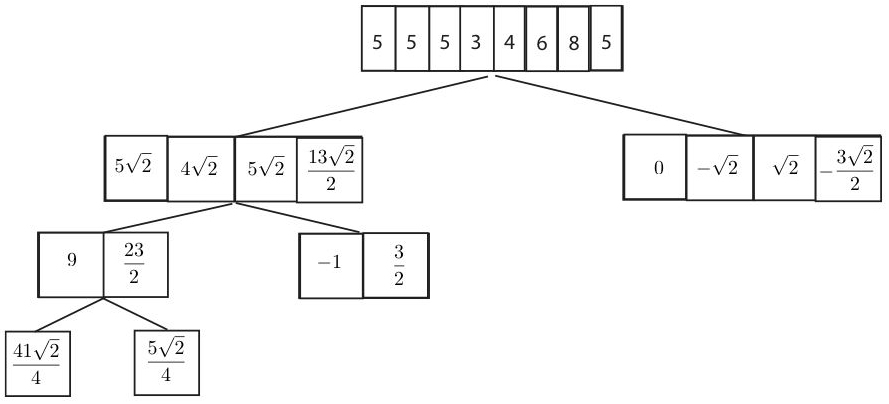
\includegraphics [width=6in]{mraexample2.jpg}
\caption{The Haar Transform performed a sample function show each step of the transform in multi-resolution analysis }
\label{nummra}
\end{figure}

For MRA, the analysis is continued on the average branch.  The difference branch is unchanged.  This procedure is repeated on the average branch.   The stopping point is determined by the size of array.  The finite limit, $n$, is 
\begin{equation} \label{eqn:treeheight} \displaystyle
n = \lceil\log_2 \left|S\right|\rceil
\end{equation}
where $\left|S\right|$ is the size of the array.

Once completed, the arrays are joined into an array which is the same
size as the original.  The energy is generally concentrated at the
beginning of the array.  Also, the energy of the array tends to be
ordered from strongest to weakest.  Terms representing change are kept
as pairs to each section.

Notice that the fine difference terms are left alone, and the dynamics
of the function in the time domain are accentuated.  Likewise the
lower frequency components are separated allowing a closer analysis in
both position and frequency.


\subsection {MRE Example}

Like MRA, MRE starts with an original array, and applies a wavelet transform to that array.  The decomposition is also represented by binary tree, with an average and difference branch.  The limit and height of the tree, $n$, remains the same as equation \ref{eqn:treeheight}.

\begin{figure}
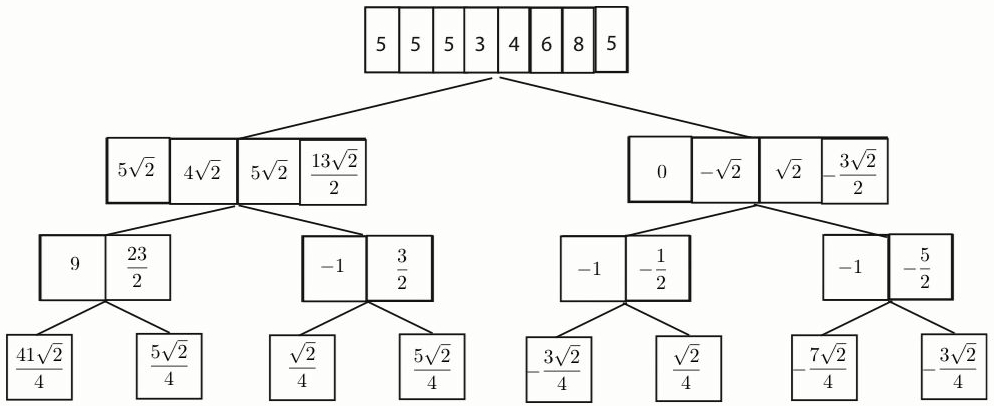
\includegraphics [width=6in]{numexample01_2.jpg}
\caption{The Haar Transform performed a sample function show each step of the transform in multi-resolution expansion }
\label{nummre}
\end{figure}

What is not the same is how the wavelet transform is reapplied.  In
addition to being applied on the average branch again, but the wavelet
transform is also applied to the difference branch also.  An example
is provided in Figure \ref{nummre}. The sub arrays are reinserted into
the array in order from the left branch to the right branch.

In the time and frequency analogues, each transformation filters the
array with high pass and low pass filter.  The frequency width of
these sub arrays is proportional to length of the original array.  The
center frequency is relative to the position of the sub-array within
the array.  The lowest frequency components are on the average side of
the array, and the highest frequency components are on the difference
section of the array.  One special case exists for arrays of length
$2^n$.  If the array is of length $2^n$, then the full MRE yields
entire frequency domain.  In case that the array is of odd size larger
than one, then the array must be padded and then normal decomposition
can continue.

  
\subsection {$\psi^n$ Expansion}
One other form of the multi-resolution expansion that can be used is almost trivial by its nature, $\psi^n$ expansion.  This particular form has the same branches as the MRE.  However, the sub arrays are place back in the array in a different order.    Figure \ref{numpsin} illustrates the difference in ordering from the $\psi^n$ form and the MRE form.    This form makes for a difficult analysis of time and frequency components, but contributes advantages linear operations.
\begin{figure}
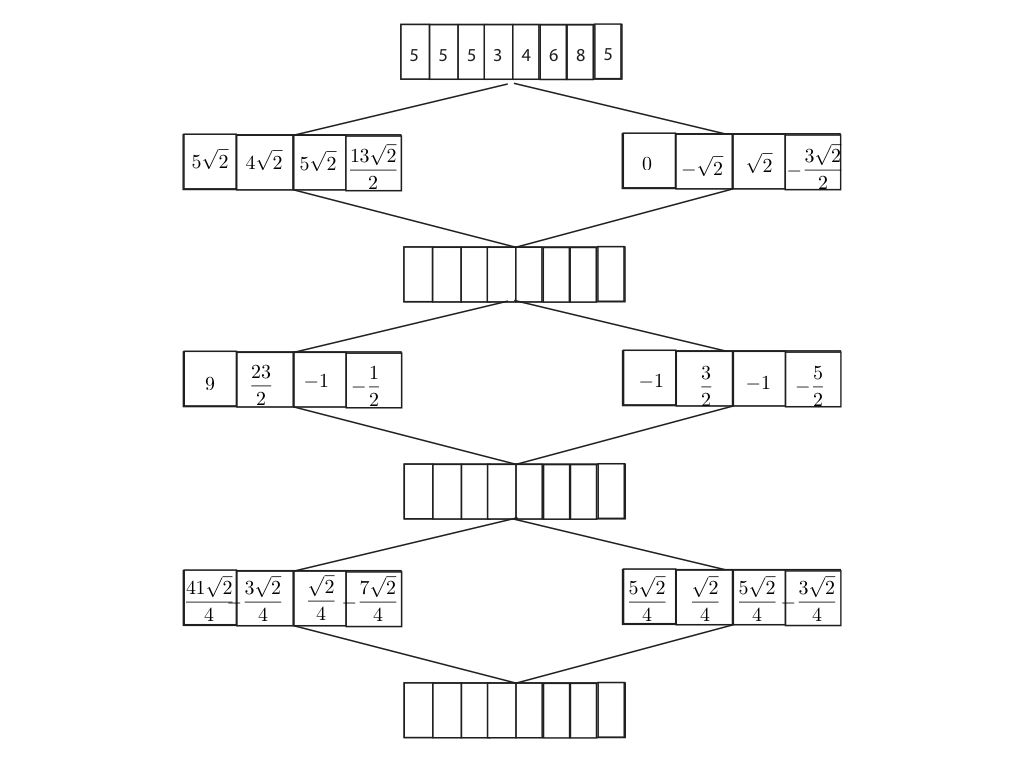
\includegraphics [width=6in]{psinexpansion.jpg}
\caption{The Haar Transform performed a sample function show each step of the transform in $\psi^n$ expansion }
\label{numpsin}
\end{figure}

\section{Implementation of the Wavelet Transform} \label{sec:implementation}

As stated before, the wavelet transform is defined in terms of average
and difference components. A signal is taken and transformed into the
two base objects.  Typically, the transform has the form $S\rightarrow
(A'|D')$ where $S$ is the original signal, $A$ is the average component,
$D$ is the difference component and $(A'|D')$ the signal $A'$
concatenated with $D'$.  This transformation can be modeled with the
convolution operator. Despite the decomposition of the signal into the
two components, the original signal can be reconstructed.

Many mathematicians such as Walker \cite{walker}, use a form that
eliminates half of the values. Thus a form can be defined which has
the same number of elements as the original.  The rules for choosing
the member elements are dependent on the wavelet filter choice. 
Another useful property of wavelets via convolution is the simplicity
of the operation. The general case works for all.  Such an algorithm
requires one nested loop as seen in Algorithm \ref{alg:convolution}.

\begin{algorithm}
\caption{Convolution of two signals $x(\cdot)$ and $h(\cdot)$.}
\label{alg:convolution}
\begin{algorithmic}
\STATE $y_i = 0$ $\forall i \in (0,M-1)$
\FOR{$i=0$ to $M-1$}
\FOR{$j=0$ to $N-1$}
\STATE $n=i-j$
\IF{$(0 \leq n < M)$}
\STATE$y(i) \  += \ x(j)\cdot h(n)$
\ENDIF
\ENDFOR
\ENDFOR
\end{algorithmic}
\end{algorithm}

This filter simply equates to the mathematical function
\[
y(k) = (x\ast h)(k) = \sum_{l}x(l)h(k-l)
\]
which is the convolution operation. It is obvious
that the operation is $O(NM)$ . For practical
use, the filter is made smaller than the actual signal being
analyzed. In some cases, the filter may be much smalled than the
signal. Filter size matters in extracting features from the original
signal.

To perform a wavelet transform via convolution, the signal is first
convolved with the average operator and then with the difference
operator.This can be represented by
\[
A = S \ast \phi 
\qquad \mbox{ and } \qquad
D = S \ast \psi.
\]
where $\phi$ is the mother wavelet and $\psi$ is the difference wavelet.

\section{The 2D Wavelet Transform} \label{sec:2Dwavelet}

For the 2D Wavelet Transform, it has to be determined how to represent
average and difference components. This can be done by creating one
average components and three difference component - vertical,
horizontal and diagonal. This can be used in a multiresolution fashion
to provide several levels of decomposition. 

A complete transform method returns a result matrix which is the same
size as the source matrix. The result contains the four
components. Each component resides on 4 corners of the matrix. Given a
matrix $B$, the transform is to yield the following form:
\[ 
B \Rightarrow 
\left(
\begin{array}{cc}
H & D \\ 
A & V
\end{array}
\right)
\]
where $A$ is the average component, $H$ is the horizontal component,
$V$ is the vertical component, and $D$ is the difference
component. There is another form which is also used as an example:
\[
B \Rightarrow 
\left(
\begin{array}{cc}
A & V \\ 
H & D
\end{array}
\right)
.\]
The first version is simple in concept, but provides a few more
possibilities for error and confusion.  Regardless of the case, the
four components have the following definitions:
\begin{enumerate}
\item Average component: produced by filtering the row vectors and the column vectors with the averaging filter.
\item Vertical Component:  produced by applying the average filter to the column vectors and the difference filter to the row vectors.
\item Horizontal component: produced by applying the average filter to the row vectors and the difference to the column vectors.
\item Diagonal component: produced by applying the difference filter to both the row and column vectors.  
\end{enumerate}

\subsection {Multi-Resolution in two-dimensions} 

Three methods are presented for decomposing 2D matrices --- 2D MRE, 2D
MRA and 2D $\psi^n$ Expansion. The first of these methods for matrices
is the 2D MRE.  In this form, the wavelet transform is applied
recursively to each of the sub-matrices.  The inverse of this MRE
applies the inverse wavelet transform is applied to the lowest level
adjacent sub-matrices.

The 2-D MRA is a special case of the 2-D MRE.  The application of the
wavelet transform is only applied to the average sub-matrix, only.
This method is also called wavelet pyramids.

The $\psi^n$ is rather more simple to implement, but is harder to
analyze.  In this case, the wavelet transform is simply reapplied to
the whole matrix.  The result of this method contains the same
elements as the 2-D MRE (wavelet transform full decomposition).
However, the arrangement of the elements is not the same.  This
arrangement will be used for matrix multiplication.

The method for visualizing 2D MRE and 2D MRA is similar to the
one-dimensional version.  Here a quadtree is used instead.  The four
branches represent the four sub-matrix types (average, vertical,
horizontal, and diagonal).  The rules for this tree is similar for the
1D wavelet transform binary tree.

The following are rules for the 2D wavelet transform quad tree in MRA.
\begin{itemize}
\item Transforms are only applied to leaves.
\item Transforms are only allowed on the root or average leaves.
\item If a node is not a leaf, then a wavelet transformation has already been performed and is not permitted to be reapplied.
\item If the leaf is a vertical, diagonal or horizontal term, then a transformation is not allowed.
\item The maximum height of this tree is 
$n = \min \left( \lceil N_r \rceil, \lceil N_c \rceil \right)$,
where $N_r$ is the number of rows in the matrix and $N_c$ is the number of columns in the matrix.
\end{itemize}   

MRE extends this idea by considering the difference leaves, also.  The rules for the 2D wavelet transform quad tree in MRA are below.
\begin{itemize}
\item Transforms are only applied to leaves.
\item If a node is not a leaf, then a wavelet transformation has already been performed and is not permitted to be reapplied.
\item The maximum height of this tree is 
$n = \min \left( \lceil N_r \rceil, \lceil N_c \rceil \right)$,
where $N_r$ is the number of rows in the matrix and $N_c$ is the number of columns in the matrix.
\end{itemize}   



%\subsection{Proof of Concept}
\subsection{Methods of Implementation}
Two methods of convolving a matrix are easily conceived.  First is to
use 1D wavelet.  The other is to apply the convolution scheme
straight to the matrix. Included in the wavelet experiment are both.
Realistically, both can and do achieve the same result.  However, the
direct method achieves speed advantages by the lack of overhead.  The
direct method only stores a temporary vector resident in memory.  Also,
there are two fewer transfers per row and column.

\subsubsection{1D to 2D Method}

Both rows 1D and 2D and columns 1D and 2D transform are performed
similarly.  The obvious difference is the indexing of rows and
columns.

\begin{algorithm}
\caption{Wavelet Row Transform}
\begin{algorithmic}
\REQUIRE Wavelet Transform, , and Wavelet Pair ($\psi$ and $\phi$)
\REQUIRE Matrix, $S \in {\mathbb R}^{N\times M}$
\FOR{$i = 0$ to $N-1$}
\STATE $R = S.getRow(i)$
\STATE $S.row(i) = \left[ R \ast \phi, R \ast \psi \right]$
\ENDFOR
\end{algorithmic}
\end{algorithm}

This principle of this algorithm is simple.  Only three intuitive steps are necessary per row or column.  Two of these steps are array transfers (row/column transfer to an array).  These arrays are fed into the 1D transforms.  

However, the 1D wavelet transform itself includes a series of memory allocation and deallocation operations.  Each memory call is at the minimum a system call.  

\subsubsection {Vector - Matrix Method}
The principle of this algorithm is more complicated.  All functionality, such as convolution, is built into the method.  There are fewer calls and passing of structures to external functions to compute the transform.  

This method has a few givens.  The source matrix, the Haar average filter, and the Haar difference filter are given arguments.  The result argument is the return argument.    The transform signals sub-function row transforms and column transforms to perform the work.  

The algorithm is as follows for the row transform (and is similar for the column transform):  

\begin{algorithm}
\caption{Wavelet Transform: Vector - Matrix Method: Row Transform }
\label{vmmethodrow}
\begin{algorithmic}
\REQUIRE  Wavelet Pair
\REQUIRE Temporary Vector $S$
\REQUIRE Matrix, $A \in {\mathbb R}^{M\times N}$
\FOR{$i = 0$ to $M$}
\STATE load $S$ from $A_i$ where $A_i$ is the row vector at row $i$
\STATE $S \stackrel{\psi_1}{\to} R$
\STATE Load $R$ into result matrix $\alpha$ at $\alpha_i$
\ENDFOR
\STATE Return $\alpha$
\end{algorithmic}
\end{algorithm}

\begin{algorithm}
\caption{Wavelet Transform: Vector - Matrix Method: Column Transform }
\label{vmmethodcol}
\begin{algorithmic}
\REQUIRE  Wavelet Pair
\REQUIRE Temporary Vector $S$
\REQUIRE Matrix, $A \in {\mathbb R}^{M\times N}$
\FOR{$j = 0$ to $N$}
\STATE load $S$ from $A_j$ where $A_i$ is the column vector at column $j$
\STATE $S \stackrel{\psi_1}{\to} R$
\STATE Load $R$ into result matrix $\alpha$ at $\alpha_j$
\ENDFOR
\STATE Return $\alpha$
\end{algorithmic}
\end{algorithm}

To perform a wavelet transform with this method, the driving wavelet transform method calls on of the wavelet transform methods and feeds the results into the other.  In the implementation used for this thesis, the row transform is called first,  then its results $\alpha$ are fed into the column transform as the column transforms $A$.  The results from the column transform are returned as the wavelet transform of the original matrix.  


\subsection{2-D MRA: Wavelet Pyramids}

This version of the wavelet transform (multiresolution) uses private members of the class $(hA, hD, xD/yD, xA/yA)$.  Both Haar filters are maintained this way.  Also both row and column transforms have average and difference myVector classes for temporary storage.   All of these members are allocated and destroyed by the wavelet transform method itself.   The simplified algorithm of the row transform is shown in Algorithm \ref{wpmethodrow}, and the column transform is shown in Algorithm \ref{wpmethodcol}.

\begin{algorithm}
\caption{Wavelet Transform: Wavelet Pyramid Method: Row Transform }
\label{wpmethodrow}
\begin{algorithmic}
\REQUIRE  Wavelet Pair $hA$ and $hD$ of length $w_l$
\REQUIRE Temporary Vector $S$
\REQUIRE Matrix, $A \in {\mathbb R}^{M\times N}$
\REQUIRE Limits of Rows and Columns to traverse: $M'$ and $N'$
%\REQUIRE Row index $i$
\REQUIRE Temporary vectors $xA$ and $xD$ for row Average vector and row Difference Vector.
\STATE Initialize vector $xA$ and $xD$
\FOR {$i = 0$ to $M'$}
\STATE Initialize $xA$ and $xD$
\FOR{$k = 0$ to $N'$}
\FOR {$l=0$ to $w_l$}
\STATE $n = k - l$
\IF {$n \in [0,N']$}
\STATE $xA_k = A_{i,n} \cdot hA_l$
\STATE $xD_k = A_{i,n} \cdot hD_l$
\ENDIF
\ENDFOR
\ENDFOR
\STATE Transfer to $\alpha$.  $\alpha_i  \leftarrow xA'|xD'$
\ENDFOR
\STATE Return $\alpha$
\end{algorithmic}
\end{algorithm}

\begin{algorithm}
\caption{Wavelet Transform: Wavelet Pyramid Method: Column Transform }
\label{wpmethodcol}
\begin{algorithmic}
\REQUIRE  Wavelet Pair $hA$ and $hD$ of length $w_l$
\REQUIRE Temporary Vector $S$
\REQUIRE Matrix, $A \in {\mathbb R}^{M\times N}$
\REQUIRE Limits of Rows and Columns to traverse: $M'$ and $N'$
%\REQUIRE Row index $i$
\REQUIRE Temporary vectors $yA$ and $yD$ for column Average vector and column Difference Vector.

\FOR {$j = 0$ to $N'$}
\STATE Initialize $yA$ and $yD$
\FOR{$k = 0$ to $M'$}
\FOR {$l=0$ to $w_l$}
\STATE $n = k - l$
\IF {$n \in [0,M']$}
\STATE $yA_k = A_{n,j} \cdot hA_l$
\STATE $yD_k = A_{n,j} \cdot hD_l$
\ENDIF
\ENDFOR
\ENDFOR
\STATE Transfer to $\alpha$.  $\alpha_j  \leftarrow yA'|yD'$
\ENDFOR
\STATE Return $\alpha$
\end{algorithmic}
\end{algorithm}

\begin{algorithm}
\caption{Wavelet Transform: Wavelet Pyramid Method: Driving Transform }
\label{wpmethod}
\begin{algorithmic}
\REQUIRE  Wavelet Pair $hA$ and $hD$ of length $w_l$
\REQUIRE Matrix $A$ of size $M\times N$
\REQUIRE Number of resolutions, $r$
\STATE Initialize matrix $\alpha$ to $M\times N$ and set equal to $A$
\STATE Initialize matrix $\beta$ to $M \times N$ and set equal to zero.
\FOR {$k = 0$ to $r$}
\STATE $M' = \frac{M}{2^k}$
\STATE $N' = \frac{N}{2^k}$
\STATE call row transform for matrix $\alpha$, with dimension limits $M'$ , $N'$ store in $\beta$
\STATE call column transform for matrix $\beta$, with dimension limits $M'$ , $N'$ store in $\alpha$
\ENDFOR
\STATE Return $\alpha$ as result
\end{algorithmic}
\end{algorithm}



Note: $A_i$ names the row vectors and $A_j$ names the column vectors, and $A_{i,j}$ is the element from the $i^{th}$ row and $j^{th}$ column.

The computational cost of this algorithm is $c \cdot C_\psi$  where $C_\psi$ is the cost of the wavelet transform at large, and $n$ is the number of resolutions performed.  The reason for this constant is that the size of the matrix being transformed shrinks by a factor of $2$ each time.  There may be additional overhead for the setup of the matrices, and transfer of matrix $S$ to $T$, which is $N^2$.  Since $C_\psi \propto O(N^2)$, and $c$ is based on $\log_2(N)$, then this a cost of another constant multiplied by $O(\sum\limits_{k=0}^{log_2(N)} \frac{1}{k^2}N^2))$.

\subsection {2-D MRE via Quad Tree}
There are two ways to implement the 2-D MRE and it depends on if other stopping conditions are desired.  The one stopping condition of size can be handled in a simple loop.  To enforce an energy limit stop, then a means to stop any further transforms on that branch must be used.   Two such means exist.   One way is to mark that branch and do so to its children.  Another way is to use a queue structure to designate nodes to be transform.  If the node represents a stopping condition, simply do not enter that node into the queue. 

In either case, the matrix information can be stored in this quad-tree.  Either by referencing position within the working matrix, or by storing a matrix in the node itself.  In this thesis, references were used for space efficiency.  However, the storage of the matrices in the nodes is just as valid.  Also a hybrid of only storing the final matrices in the leaves is acceptable as well.  

As stated, a straightforward loop can acquire the full decomposition.  The limit of the times required for is defined $v_l = 4^{r-1} $  where $r$ is the height of the quad-tree.  In this implementation, the quad tree is implemented in an array, and those properties are exploited in using a simple for loop to perform the 2-D MRE.
%    for ( index = r.id; index < length4; index++)
%    {
%        qtree->gotoNode(index);
%        qtree->getNode (temp);
%        selfRowWXform(temp);
%        selfColWXform(temp);
%        getSstats(temp);
\begin{algorithm}
\caption{Wavelet Transform: MRE Quad Tree Loop }
\label{mreqtloop}
\begin{algorithmic}
\REQUIRE Wavelet Transform, $\psi$, and Wavelet Pair
\REQUIRE Matrix, $S \in {\mathbb R}^{N\times M}$
\FOR{$i = 0$ to $v_l$}
\STATE draw $S$ from quad-tree at index $i$
\STATE $S \stackrel{\psi_r}{\to} T$
\STATE $T \stackrel{\psi_c}{\to} X$
\STATE Wavelet Split and Store $X$ in branch children.
\ENDFOR
\end{algorithmic}
\end{algorithm}

Note on Algorithm \ref{mreqtloop} that the Wavelet Split and Store operation splits the matrix $X$ into its four sub-matrices (average, horizontal, vertical, and diagonal) and stores them in their appropriate spot in the tree.  Thus every-time that $S$ is loaded a leaf branch of the tree is loaded to be transformed.  

The queue based 2-D MRE with a quad-tree is a bit more complicated.  The queue must be loaded with the root, then operation may be allowed to proceed.  The end condition is when the queue is empty.  Rules for loading the queue is must force the leaves on the last level to be ineligible for loading.    Otherwise, the loop will never stop and segmentation fault is likely to arise.  Energy rules and other arbitrary rules may also be imposed, but they are not as critical as the leaf limit rule.  For this example, refer to Algorithm \ref{wavemreloop}.
\begin{algorithm}
\caption {Wavelet Transform: MRE with queue controlled visits of the Quad Tree}
\label{wavemreloop}
\begin {algorithmic}
\REQUIRE Wavelet Transform, MRE, and wavelet pair ($\psi$ and $\phi$)
\REQUIRE Matrix $S$ 
\STATE {Insert root node representing the whole matrix in the queue.}
\WHILE {as long as queue is not empty} 
\STATE Get the next element from the queue, and load matrix $S$
\STATE $S \stackrel{\psi_r}{\to} T$
\STATE $T \stackrel{\psi_c}{\to} X$
\STATE Check $X$ for terminating conditions
\STATE if $X$ does not have a terminating condition store $X$'s four sections into the branch children of node $S$.  Store theses children nodes in the queue in order of average, vertical, horizontal, and difference.

\ENDWHILE
\end {algorithmic}
\end{algorithm}
The computational cost of this algorithm $n\cdot C_\psi$  where $C_\psi$ is the cost of the wavelet transform at large, and $n$ is the number of resolutions performed.  In some special cases, the cost may be slightly to significantly less if additional termination rules are applied.  The reduced size of the sub-matrices is canceled by quantity of sub-matrices to transform.  There may be additional overhead for the setup of the matrices.  Since $C_\psi \propto O(N^2)$, and $n$ is based on $\log_2(N)$ then this has a cost on the order of $N^2\log_2(N)$ also.  

%{
%    quadnode temp, temp2, a,v,h,d;
%    int ai, vi, hi, di;
%    queue->put (r);
%    int length = resolution;
%    int length4 = resolution / 4;
%    while (!queue->empty())
%    {
%        queue->get(temp);
%        if (qtree->gotoNode(temp.id) & (( temp.id ) < length4 ))
%            selfRowWXform(temp);
%            selfColWXform(temp);
%            getSstats (a);
%            getSstats (v);
%            getSstats (h);
%            getSstats (d);
%            ai = qtree->getA();
%            vi = qtree->getV();
%            hi = qtree->getH();
%            di = qtree->getD();
%            if ( ai < length4) {
%               qtree->getStats(S, ai);
%                qtree->getNode (ai, a);
%                queue->put(a);
%            }
%            if ( vi < length4) {
%                qtree->getStats(S, vi );
%                qtree->getNode (vi, v);
%                queue->put(v);
%            }
%            if ( hi < length4) {
%                qtree->getStats(S, hi );
%                qtree->getNode (hi, h);
%                queue->put(h);
%            }
%            if ( di <= length4) {
%                qtree->getStats(S, di );
%                qtree->getNode (di, d);
%                queue->put(d);



\subsection {2-D $\psi^n$ Implementation}
As stated the $\psi^n$ expansion is simpler to implement, but produces a matrix that is harder to analyze for features.  However, it is scientific merit since it is literally a wavelet transform of a wavelet transform.   Also, the limits imposed on the MRA and MRE for tree height are not required, but are rather a good idea.  A good practical limit would be for the resolution limit to be defined $n =\log_2 |S| -1$  where $|S|$ is the size of the the matrix S.  For this example, refer to Algorithm \ref{wavepsiloop}.
\begin{algorithm}
\caption {Wavelet Transform: MRE with queue controlled visits of the Quad Tree}
\label{wavepsiloop}
\begin {algorithmic}
\REQUIRE Wavelet Transform, MRE, and wavelet pair ($\psi$ and $\phi$)
\REQUIRE Matrix $S$ 
\STATE {Load $S$ into temporary matrix $T$}
\FOR {$i = 1$ to $n$}
\STATE {$T \stackrel{\psi_c}{\to} X$}
\STATE {$X \stackrel{\psi_r}{\to} T$}
\ENDFOR 
\STATE {return $T$ as the transformed matrix}

\end {algorithmic}
\end{algorithm}

The computational cost of this algorithm $n\cdot C_\psi$  where $C_\psi$ is the cost of the wavelet transform at large, and $n$ is the number of resolutions performed.  There may be additional overhead for the setup of the matrices, and transfer of matrix $S$ to $T$, which is $N^2$.  Since $C_\psi \propto O(N^2)$ then this has a cost on the order of $O(N^2\log_2(N))$.

%\section {Computational Cost}

%This should given after each algorithm.



%The cost of this algorithm is computed first for each row and each column.  This value is used to compute the cost of the matrix. The cost of computing the matrix is used to compute the cost of the multiresolution steps.   Per row the cost is $3K$, where $K$ is the number of columns.  Per column the cost is $3L$, where $L$ is the number of rows.  For the whole matrix, one resolution costs $6KL$ operations to compute the wavelet transform.    

%Per resolution with MRA, the rows and columns shrink by $2^i $ for each resolution, i, performed.  The limit of this cost equals $12KL$ operations.  If the values of $K$ and $L$ are relatively large, then it can be said that the order is $12N^2$ where $N$ is the worst case of the length or width of the matrix.    

%With either $psi^n$ expansion or MRE, the wavelet transform is reapplied to the whole matrix.  In the case of the $psi^n$ 

%Stopped at this point April 10, 2003



%\begin{thebibliography}{99}
%\bibitem {ChuiIntro} Charles Chui \textsl {An Introduction to Wavelets} published by Academic Press San Diego, CA 92101-4495 copyright 1992

%\bibitem{matrix01}Howard L. Resnikoff. and Raymond O. Wells, Jr. \textsl {Wavelet Analysis: The Scalable Structure of Information}  copyright Springer-Verlag New York, Inc.  New York, NY 10010, USA, 1998
%\bibitem{walker}James Walker \textsl {A Primer on Wavelets and Their Scientific Applications}
%copyright Chapman \& Hall/CRC : Boca Raton, FL, USA, 1999
%\bibitem{tabor}Gavin Tabor \textsl {Wavelets - The Idiots Guide} http://monet.me.ic.ac.uk/people/gavin/java/waveletDemos.html
%\bibitem {graps} Amara Graps \textsl {Introduction to Wavelets} http://www.amara.com/current/wavelet.html 

%\bibitem {appliedmethods} Singiresu S. Rao \textsl{Applied Numerical Methods for Engineers and Scientists}  published Prentice Hall Upper Saddle River, NJ 07458 copyright  2002
%\bibitem {numrecipies} William H. Press, Saul A. Teukolsky, William T. Vetterling, and Brian P. Flannery 

%\textsl {Numerical Methods in C}
%Published by the Press Syndicate of the University of Cambridge The Pitt Building, Trumpington Street, Cambridge CB2 1RP%40 West 20th Street, New York, NY 10011-4211, USA
%Copyright Cambridge University Press 1988, 1992

%\bibitem {bvpbeylkin}  G. Beylkin \textsl{On wavelet-based algorithms for solving differential equations}

%\bibitem {amsbeylkin}  G. Beylkin \textsl{Wavelets and Fast Numerical Algorithms}

%\bibitem {fwtnal} G. Beylkin, R. Coifman, and V. Rokhlin \textsl {Fast Wavelet Transforms and Numerical Algorithms I, Article in Communications on pure and applied mathematics} copyright 1991 Wiley, New York

%\bibitem {mwabeylkin}  G. Beylkin, D. Gines and L. Vozovoi \textsl{Adaptive Solution of Partial Differential Equations in Multiwavelet Bases }

%\bibitem {PDEfSE} Stanly J. Farlow \textsl{Partial Differential Equations for Scientists and Engineers} copywrite 1993 Dover Publications, Inc Mineola, N.Y. 11501

%\bibitem {spiegel} Murray R. Spiegel, \textsl { Theory and Problems of Advanced Mathematics for Engineers and Scientist} copy-write 1996 McGraw-Hill 

%\bibitem {tools} Stephane Jaffard, Yves Meyer, and Robert D. Ryan \textsl {Wavelets: Tools for Science and Technology} copyright 2001 by the Society for Industrial and Applied Mathematics Philadelphia, PA 19104-2688

%\bibitem {victor} Mladen Victor Wickerhauser \textsl {Adapted Wavelet Analysis from Theory to Software} copyright 2001 by the Society for Industrial and Applied Mathematics Philadelphia, PA 19104-2688

%\bibitem En-Bing Lin and Zhengchu Xiao \textsl {Multiwavelet Solutions for the Dirichlet Problem} Department of Mathematics, University of Toledo; Toledo, OH 43606, USA

%\bibitem Tian-Xiao He \textsl {Wavelet Analysis and Multiresolution Methods (Lecture Notes in Pure and Applied Mathematics} published Marcel Dekker, Inc.  New York, NY 10016 copyright 2000

%\bibitem {ChuiIntro} Charles Chui \textsl {An Introduction to Wavelets} published by Academic Press San Diego, CA 92101-4495 copyright 1992


%\end{thebibliography}

% \end{document}

 
